%!TEX root = ../../../report.tex

\subsection{Dataflow}

When designing an energy efficient system, dataflow is of great importance since
data movement can cost a lot of energy. The software on the MCU
has been designed to minimize the number of data transfers. When
possible, DMA is utilized to move the data while running the MCU in a low power
mode. Dataflow is divided into four phases, as shown in figure
\ref{fig:sw_transfer_phases}.

In phase 1, the MCU retrieves samples from an input device. These samples
are then transferred to the \textit{ChaosM} in phase 2. Processed samples are transferred back to the MCU in phase 3, and in the
last phase, the MCU forwards the data to an output device. All these
phases are executed concurrently to ensure a constant flow of samples.

\begin{figure}[H]
	\centerline{
	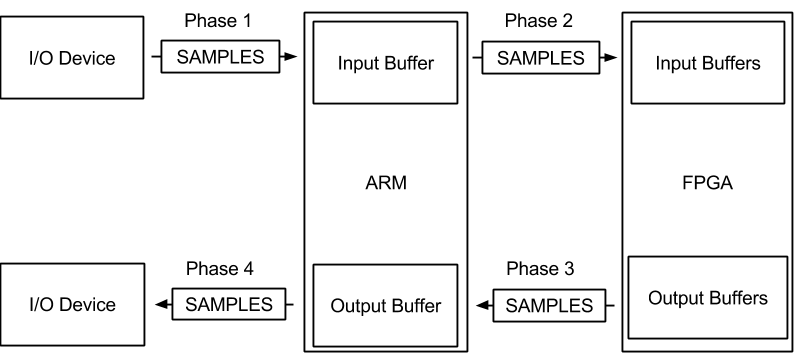
\includegraphics[width=400px]{figures/sw/transfer-phases.png}}
	\caption{Transfer Phases}
	\label{fig:sw_transfer_phases}
\end{figure}
\FloatBarrier


\subsubsection{Direct Memory Access}

Direct Memory Access (DMA) provides the ability to move data without
intervention from the CPU. This is used extensively to move data while the
MCU is running in a low energy mode. The CPU on the MCU is only used to
configure and refresh the DMA channels in between transfers. The MCU provides 12
independent DMA channels which can move data between peripherals, internal RAM,
and devices connected to EBI like the FPGA.

% \input{figures/sw/ram-fpga-ram}

\subsubsection{Deinterleaving the samples}

When reading from either a WAV file or the ADC, samples from the stereo channels
are interleaved. The \textit{ChaosM} handles each channel in a separate pipeline as shown
in Figure \ref{fig:pipeline_architecture}. When reading the samples they have to be
deinterleaved. Deinterleaving is the process of splitting the samples for each
channel into separate streams. The complementary operation of interleaving the
samples is performed before the samples are moved to the output peripherals. This is
illustrated in Figure~\ref{fig:interleaving}

\begin{figure}[H]
    \centering
    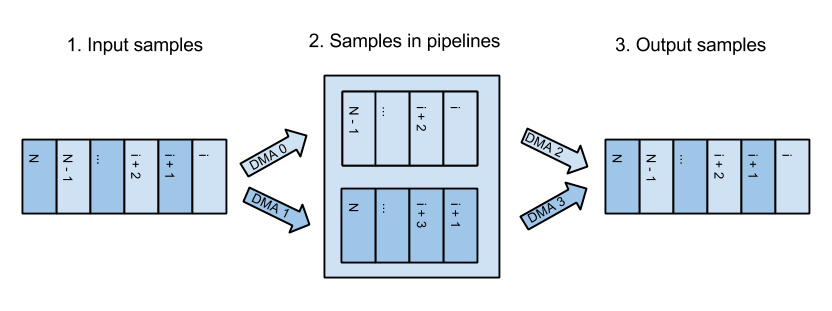
\includegraphics[width=1\textwidth]{figures/sw/interleaving-of-samples.png}
    \caption{Interleaving and deinterleaving of samples}
    \label{fig:interleaving}
\end{figure}

The interleaving and deinterleaving operations are either done by the DMA for
energy efficiency purposes, or the CPU. If the operation is performed by the
CPU, the gains of speed and data-transfer analysis can be tested. Depending on
the different types of input sources, the CPU might be needed, while on others a
more energy efficient implementation through the use of DMA may be used.
Comparisons of the two implementations are included in the results section.

The samples are deinterleaved in the DMA implementation by letting two DMA
channels read from the same source and write the correct channel into the the
correct pipeline for the correct channel. The first DMA copies the samples for
the left stereo channel, and starts without a offset. The second DMA copies the
samples for the right stereo channel and starts with an offset of one sample.
Both DMAs read every other sample and writes them continuously to the FPGA input
buffers.

In the code, this is set up with the DMA interface in {\bf emlib}, by
configuring the DMA Descriptor. This is implemented with two
version. One using only the CPU and one using DMA transfers while the CPU is
sleeping.

To understand what this will result in, imagine two pointers, {\bf dst} and {\bf
src}. At each iteration {\bf size} bytes are copied from {\bf src} to {\bf dst}.
After each iterations the {\bf src} pointer is incremented by {\bf srcInc} bytes
and the {\bf dst} pointer is incremented by {\bf dstInc}.

After the DMA channel is configured with a descriptor, it can be started with a
a source pointer, destination pointer, and the number of transfers to be
executed. When the transfer has finished the CPU is interrupted and can start
the next transfer.

The interleaving process on the output side of the FPGA works in the same way.
The DMA reading the audio pipeline containing the left stereo channel, writes
the samples to even numbered addresses in the memory, while the DMA reading the
right audio pipeline channel writes to odd numbered addresses.

Additionally, a DMA is assigned for each ADC and DAC whenever they are used as
input and output. When a SDCard is used, the contents of the files are read and
written directly to and from RAM by the CPU.

\subsubsection{Peripherals}

\begin{figure}[h]
	\centering
	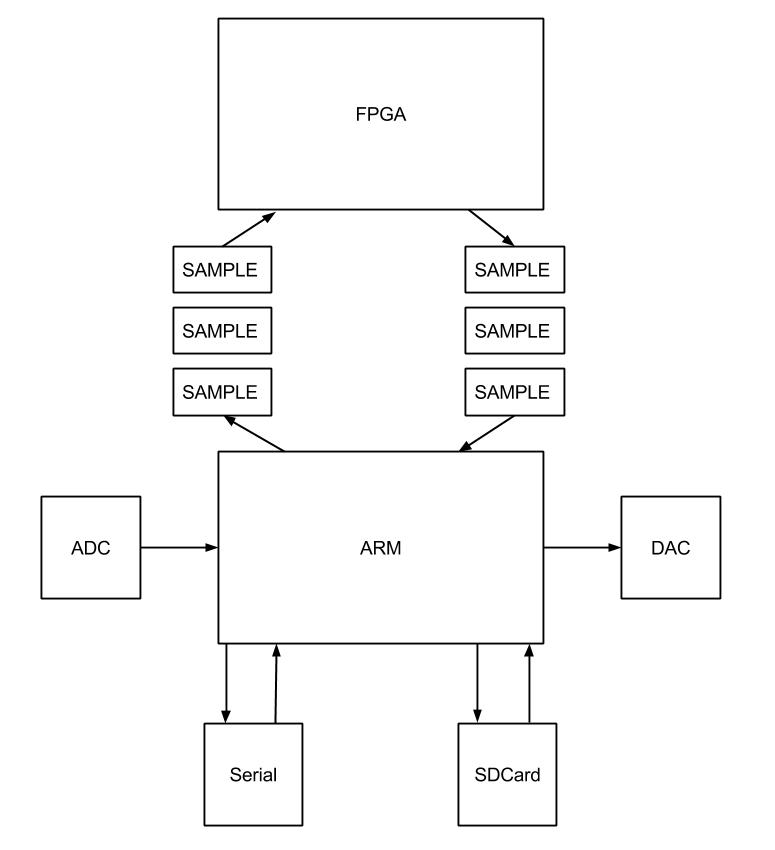
\includegraphics[height=150px]{figures/sw/sample-flow.png}
	%\begin{tikzpicture}[shorten >= 1pt, node distance=3cm, on grid, auto]
	%	\node[draw,rectangle,minimum size=2cm] (fpga) {FPGA};
	%	\node[draw,rectangle,below of=fpga,minimum size=2cm] (arm) {ARM};
	%\end{tikzpicture}
	\caption{Flow of samples}
	\label{fig:sw_sample_flow}
\end{figure}
\todo{Tikzify}


Figure \ref{fig:sw_sample_flow} show all the peripherals included in the flow of samples.
The ADC and DAC are connected to the minijack audio ports on the circuit board and directly
linked to GPIO ports on the MCU. The SDCard
is mounted on the PCB and connected to the MCU through the Serial Peripheral Interface (SPI)
bus. Lastly the FPGA is connected to the MCU on the EBI.

\subsubsection{External Bus Interface}
The MCU is connected to the FPGA and External SRAM through the EBI. The EBI bus
is initialized by the {\it emlib} software library. Utilizing
the EBI leads to a simple interface with these units since the bus is memory
mapped on the MCU. Communicating with the FPGA is done by reading and writing to memory.

\subsubsection{Serial Peripheral Interface}
The SPI bus is a general bus interface used in many embedded applications. It is used
for communicating between the MCU and the microSD memory card connected to the slot

on the PCB.

\subsubsection{General Purpose Input/Output}
To capture an audio stream from the input minijack, one GPIO pin is connected to an
ADC on the MCU. The ADC measures the the difference between the current on the pin 
and a reference voltage, usualy Vdd or Ground. 


\subsubsection{Triggering Transfers}

All the DMA transfers are triggered by the use of one clock, the sample clock.
This clock is run at the sample speed 11 kilohertz when using the DAC or ADC. Or
an arbitrary frequency when sampling from SDCard to SDCard. The clock signal is fed into
the Peripheral Reflex System \cite{prs} of the MCU and propagates
through the system using the following scheme.

\begin{figure}[H]
    \centering
    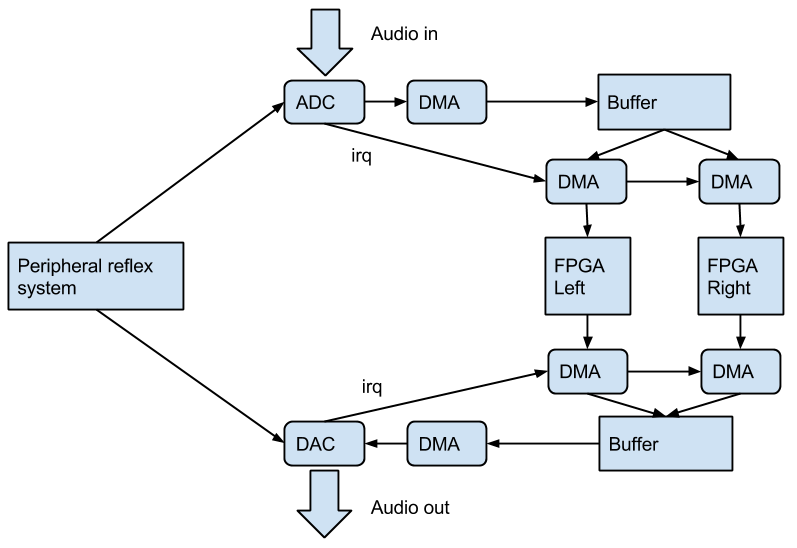
\includegraphics[width=1\textwidth]{figures/sw/dma-paths.png}
    \caption{IRQ-triggering of DMA transfers}
    \label{fig:software-stack}
\end{figure}

Here, both the DAC and ADC consumes the PRS signal originated from TIMER0. The
DMA copying from the ADC to the RAM buffer, as well as the two DMAs performing the
deinterleaving of the input samples, both receive a pulse each time the ADC has
buffered $N$ samples. They then perform a sequence of copy actions on the input
samples so that these end up inside the pipeline bufferrs of the FPGA. On the
other side, the DAC sends a pulse to the DMA that feeds it samples in conjunction
with the two DMAs performing the interleaving of the samples returned from the
FPGA pipelines.
